
\textbf{Expected Path Length (EPL):  }

% We define EPL as the expected number of time steps required for an attacker to advance from the initial state to the attack goal, and its calculation follows as a direct consequence of deriving the NR metric. That is, if the NR metric expresses the total expected time that a process starting in initial state $s_i$ will occur in transient state \(s_j\) before ultimately being absorbed, then the NR sum over all transient states for \(s_i\) will predict the total time spent in the process before absorption. To take the sum of the values in the rows of the fundamental matrix we multiply by a column of 1’s, t = N1, and the entry \(t_i\) contains the EPL value for initial state \(s_i\). 
EPL describes how long we can expect an attacker to be in our network before the target is successfully compromised. Table \ref{tab:epl_result} shows the EPL values for each model along with the path length histogram of the simulations that were run. This histogram counts how many times the simulation reached the target in exactly Path Length steps. We can infer that the higher the EPL value, the longer an attacker will attempt to advance to the target, and the more chance we have to observe and act in response [1]. The long tail on the final state histogram indicates that, in several simulations, the observed path length nearly tripled that of the other two models. We notice that, despite having significantly more available attack paths (NP(current)=6 vs NP(SDN)=3) the expected path length of the current model is actually higher than that of the SDN model. Likewise, although the SDN models  both have Shortest Path scores = 3, we have shown the resiliency of these networks to be unequal.  In doing so we demonstrate the additional insight provided by incorporating vulnerability awareness into our threat modelling and planning tools.

% \begin{figure*}[ht]
\begin{table*}[ht]
\caption{Expected Path Length Results}
\resizebox{\textwidth}{!}{%
\begin{tabular}{@{}llll@{}}
\toprule
Current & Transition & Final &  \\ \midrule
Expected Length: 9.398 & Expected Length: 8.0875 & Expected Length: 11.1405 &  \\ \bottomrule
\raisebox{-\totalheight}{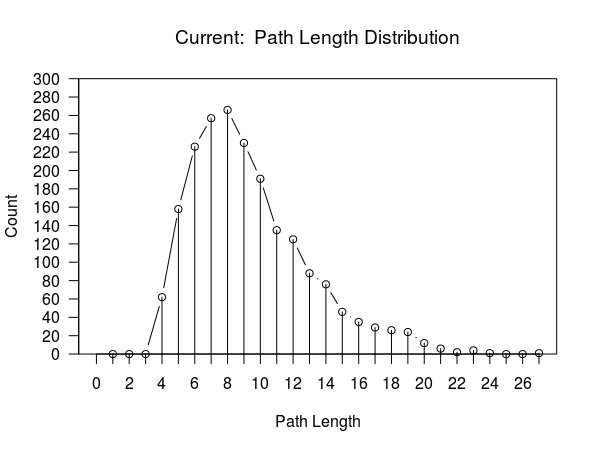
\includegraphics[width=0.3\textwidth, height=60mm]{img/pathlength_curr.png}}
      & 
\raisebox{-\totalheight}{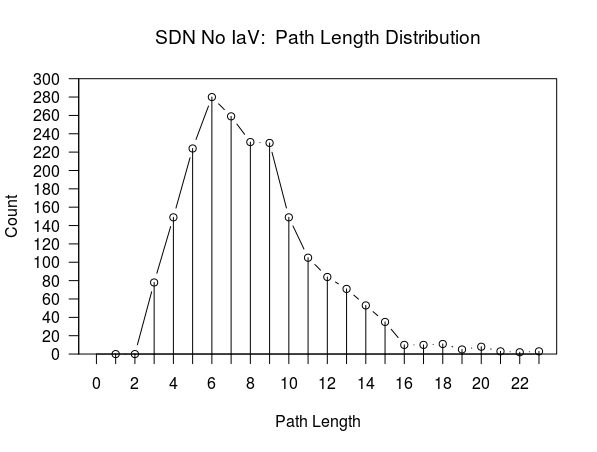
\includegraphics[width=0.3\textwidth, height=60mm]{img/pathlength_trans.png}}
&
\raisebox{-\totalheight}{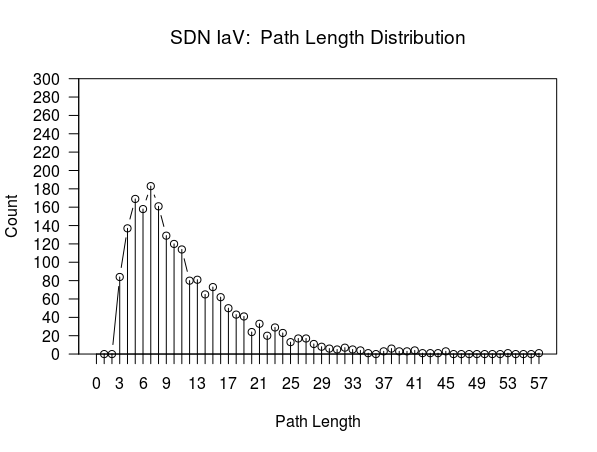
\includegraphics[width=0.3\textwidth, height=60mm]{img/pathlength_final.png}}
\\
\end{tabular}
}
\label{tab:epl_result}
\end{table*}

% \end{figure*}

 